%% LyX 2.1.4 created this file.  For more info, see http://www.lyx.org/.
%% Do not edit unless you really know what you are doing.
\documentclass[english]{article}
\usepackage[T1]{fontenc}
\usepackage[latin9]{inputenc}
\usepackage{geometry}
\geometry{verbose,tmargin=2cm,bmargin=3cm,lmargin=1.5cm,rmargin=1.5cm}
\usepackage{float}
\usepackage{mathtools}
\usepackage{amsmath}
\usepackage{amssymb}
\usepackage{graphicx}
\usepackage{tablefootnote}

\makeatletter

%%%%%%%%%%%%%%%%%%%%%%%%%%%%%% LyX specific LaTeX commands.
%% Because html converters don't know tabularnewline
\providecommand{\tabularnewline}{\\}
\floatstyle{ruled}
\newfloat{algorithm}{tbp}{loa}
\providecommand{\algorithmname}{Algorithm}
\floatname{algorithm}{\protect\algorithmname}

%%%%%%%%%%%%%%%%%%%%%%%%%%%%%% User specified LaTeX commands.
\usepackage{tikz}
\usepackage{babel}
\renewcommand{\labelitemi}{$\diamond$}
\newcommand{\T}{\rule{0pt}{2.6ex}}       % Top strut
\newcommand{\B}{\rule[-1.2ex]{0pt}{0pt}} % Bottom strut
\usepackage{algorithm,algpseudocode}

\makeatother

\usepackage{babel}
\begin{document}

\title{COMP8620: MC-AIXI-CTW\\
Group 3}


\author{Jarryd Martin, John Aslanides, Yadunandan Sannappa,\\
 Nrupendra Rao, Cheng Yu, Ryk Budzynski}


\date{October 2015}

\maketitle
We outline an implementation of Veness et al.'s Monte Carlo AIXI approximation\cite{veness-11}
(MC-AIXI-CTW), and report our simulation results on a number of toy
domains.


\section{Introduction}

Recall that the AIXI agent is defined by its actions, which for each
cycle $k$ are given by 
\[
a_{k}^{\text{AIXI}}=\arg\max_{a_{k}}\sum_{o_{k}r_{k}}\cdots\max_{a_{m}}\sum_{o_{m}r_{m}}\left[r_{k}+\dots+r_{m}\right]\xi\left(o_{1}r_{1}\dots o_{m}r_{m}|a_{1}\dots a_{m}\right),
\]


where the $o_{n}$ and $r_{n}$ are the observation and reward provided
by the environment at cycle $n$, and $\xi$ is a Bayesian mixture
model for the environment. 

Following Veness et al., we approximate $a_{k}^{\text{AIXI}}$ using
Monte Carlo tree search (upper confidence bound) to approximate the
expectimax, and we compute a mixture over variable-order Markov models
using the context-tree weighting algorithm. 

We present a lightweight C++ implementation of MC-AIXI-CTW, along
with implementations of a number of simple games: $\textsc{Pacman},\ $
$\textsc{Tic-Tac-Toe}$, $\textsc{Biased Rock-Paper-Scissor}$, $\textsc{Extended-Tiger}$,
and $\textsc{Cheesemaze}$.


\section{User Manual}

To build from source, run ${\tt g++\ *.cpp\ *.hpp\ -o\ aixi}$ \textbf{TODO
check}

To run, invoke ${\tt ./aixi\ envname}$. 


\section{MC-AIXI-CTW Implementation}


\subsection{Main loop}

For each agent-environment interaction cycle, we run the following
for each experiment:

\begin{algorithm}
\begin{algorithmic}[1]
\renewcommand{\algorithmicrequire}{\textbf{Inputs:}}
\renewcommand{\algorithmicensure}{\textbf{Outputs:}}
\While{$cycle < max\_cycles$}
\While{environment is not finished}
\State{generate $(o,r)$ from environment}
\State{update agent model with $(o,r)$}
\If{explore}
\State{$a \leftarrow randomAction()$}
\Else
\State{$a \leftarrow MCTS()$}
\Comment{Monte Carlo Tree Search}
\EndIf
\State{perform action $a$}
\State{update agent history with $a$}
\State{$cycle++$}
\EndWhile
\State{reset environment}
\EndWhile
\end{algorithmic}

\caption{Main loop.}


\end{algorithm}


The $MCTS$ algorithm follows as in Algorithms 1-4 in Veness et al.,
and is found in ${\tt search.cpp}$. Model updates are handled in
methods in ${\tt agent.cpp}$, which interfaces with the context tree
defined in ${\tt predict.cpp}$.


\subsection{Monte Carlo Tree Search (MCTS) Algorithm}


\subsubsection{High level description}

Since the environment is only partially observable, we have no explicit
notion of state; instead, we only have a history of actions and percepts
$h=\left(a_{1}o_{1}r_{1}\dots a_{n}o_{n}r_{n}\right)$. For the purposes
of choosing the optimal action, we treat each possible (hypothetical)
history as a node in the search tree, with the root being the tip
of the current (realised) history. \\

The search tree is comprised of alternate layers of decision nodes and
chance nodes with the root being a decision node. The maximum branching
possible from decision nodes is the number of available actions in the given
environment while the maximum branching possible from chance nodes is equal
to the number of possible observations times the number of possible rewards.
We do however restrict branching in general to $100$ to avoid memory issues.
This number is configurable in ${\tt search.cpp}$. \\

Each node is implicitly labelled by its history as chance nodes record the
hypothetical action taken while decision nodes record the hypothetical
observation and reward from the environment.
The expected value of each node in the search tree is equal to the
expected total (non-discounted) reward that would be accumulated from
that node, where the expectation is under the agent's current policy
and the agent's current model for the behavior of the environment. \\

Thus, for each node we keep a value estimate $\hat{V}$, and a count
of the number of times $T$ that node has been visited in search.
This is used to determine how we explore the search space using the
UCB algorithm, which, for each decision node picks (assuming $T\left(ha\right)>0$
for all actions)
\[
a_{\text{UCB}}=\arg\max_{a\in\mathcal{A}}\left\{ \frac{1}{m\left(\beta-\alpha\right)}\hat{V}\left(ha\right)+C\sqrt{\frac{\log T\left(h\right)}{T\left(ha\right)}}\right\} ,
\]

where $\mathcal{A}$ is the set of all permissible actions, $m$ is
the search horizon, $\beta-\alpha$ is the difference between the
minimal and maximal instantaneous reward, and $C$ is a parameter
controlling the propensity of the agent to explore less frequently-seen
histories. \\

Note that the expectimax is a stochastic, partially observable game
between the agent and its environment. In the following, call nodes
corresponding to agent moves `decision nodes', and nodes corresponding
to Nature's moves `chance nodes'. \\

\subsubsection{Class structure}

To represent our search nodes, we define a base ${\tt SearchNode}$
class, from which ChanceNode and DecisionNode inherit. ChanceNode
and DecisionNode each have a ${\tt sample}$ method defined on them;
each of these methods is mutually recursive. For a given node $n$,
we keep its children in a dictionary keyed on the action or (observation,reward)
used to generate each child.

\subsubsection{Code snippets}


\subsubsection{Efficiency/performance}

Between calls to ${\tt search}$, we retain much of the search tree,
pruning those nodes that are now inaccessible from the realised $(a,o,r)$
tuple that happened during the cycle. This allows us to avoid re-generating
similar search trees from similar positions. 


\subsection{Modelling using the Context Tree Weighting Method (CTW)}
The Context-Tree-Weighting Method (CTW) is a sequential universal data compression procedure for binary tree sources \cite{Willems-95}. Its computational and storage complexity are both linear in the source sequence length, making it an extremely efficient method for doing sequential binary sequence prediction. Utilising the CT data structure in the agent setting - i.e. as a mixture environment model - places two restrictions on the generality of our agent. The first is trivial, arguably no restriction at all: percepts must be encoded as binary strings, and each bit in that string must be processed sequentially. The second is more severe. The CTW algorithm performs Bayesian model averaging over all prediction suffix trees $M$ of maximum depth $D$. Hence it effectively assumes the true environment is in the class of $D$-order Markov processes. This is an enormous class, but is nonetheless much smaller than the class considered by AIXI (the class of all computable distributions). \\

Each node $n$ in the CT data structure represents a context; a suffix of the agent's history (of maximum length $D$ bits). A count is maintained for each $n$, of the number of $0$s and $1$s that have been seen from context $n$. Using these counts we recursively maintain a Krichevsky-Trofimov (KT) estimate $P_{kt}^{n}$ of the probability of the subsequence of the history seen from context $n$ to date. In our implementation we use the following update formula in terms of log probabilities for numerical reasons, (where $0_s$ and $1_s$ are the current counts): 
$$ \log{P_{kt}^n(0_s+1,1_s)} = \log{P_{kt}^n(0_s,1_s)} + \log{\frac{0_s + 0.5}{0_s + 1_s + 1}} $$
$$ \log{P_{kt}^n(0_s,1_s+1)} = \log{P_{kt}^n(0_s,1_s)} + \log{\frac{1_s + 0.5}{0_s + 1_s + 1}} $$

For each $n$ we also calculate $P_w^{n}$; which is effectively a weighted mixture of the KT estimates of $n$ and all of $n$'s descendant nodes. The formula is recursive, requiring us to first compute $P_w{\cdot}$ for the relevant leaf node (a context of length $D$), and then proceed back up along the applicable path in the context tree (updating a context of length $D-1$, then $D-2$ etc.), finishing at the root (the context $\epsilon$). Again, we put the update formula in terms of log probabilities, where $n0$ and $n1$ are the children of $n$: 

\begin{equation*}
\log{P_w^{n}} = \begin{cases} \log{P_{kt}^n} \ \ \ \ \ \ \ \ \ \ \ \text{(if $n$ is a leaf node)} \\
  \log{(P_{kt}^n + P_w^{n0}P_w^{n0})} = \log{1 + 2^{\log{(P_kt^{n}} - \log{P_w^{n0}} - \log{P_w^{n1})}}} + \log{P_w^{n0}} + \log{P_w^{n1}} -1 \ \ \ \ \ \text{(otherwise)} \end{cases}\\
\end{equation*}              
\newline
The last expression above, though ugly, is necessary for numerical reasons (discussed below). All this labour culminates in the computation of $P_w^{\epsilon}$, which is the weighted mixture mentioned above. Formally:
$$ P(x_{1:t}|a_{1:t}) \approx P_w^{\epsilon} = \sum_M{Pr(M)Pr(x_{1:t}|a_{1:t})} = \sum_M{2^{-\Gamma_D(M)}Pr(x_{1:t}|a_{1:t})}$$
where the prior probability of each suffix tree model $M$ is approximated using a cost $\Gamma_D(M)$, roughly the length of its code. Hence $M$'s with shorter description lengths are given greater weight, and thus the mixture imposes an Ockham-like penalty on complex models \cite{Veness-11} and serves as an approximation to the Solomonoff prior used by AIXI ($\sum_{q:U(q,a_{1:t}) = x_{1:t}}{2^{-l(p)}}$).

\subsubsection{High level description of algorithm}
Our implementation of the CTW has three main components: 
\begin{itemize}
\item ContextTree.update: a method for updating the CT and agent.history with a new percept;
\item ContextTree.revert: a method for reverting the CT and agent.history to their state before the last bit was observed;
\item ContextTree.genPerceptandUpdate: a method for predicting the next percept and updating the tree with it;
\end{itemize}

ContextTree.update is called when updating the CTW model with real percepts from the environment, and during the $MCTS$ action selection routine, during which the CT is updated with percepts generated by genPerceptandUpdate (below). Strictly, we have implemented two CT.update methods: one that takes as input a pair $(o_t,r_t)$ of unsigned integers, and one that takes a single bit.\\

\begin{algorithm}
\begin{algorithmic}[1]
\renewcommand{\algorithmicrequire}{\textbf{Inputs:}}
\renewcommand{\algorithmicensure}{\textbf{Outputs:}}
\State{\textbf{Inputs: } percept $x_{t}$ $=(o_t, r_t)$}
\State{encode percept $x_t$ as a bit-string $[[x_t]]$}
\For{i = 0 to \textit{($[[x_t]]$.length} - 1)}
\State{find and store \textit{context-path} \Comment{set of nodes in context tree corresponding to history-suffix preceding $x_t[i]$}}
\While{\textit{context-path} is not empty}
\Comment{begin with $n \rightarrow$ leaf, traverse back until $n \rightarrow$ root}
\State{increment counts for node $n$ with symbol $x_t[i]$}
\State{update log-KT-estimate $\log{P_{kt}^{n}}$ for node $n$}
\State{Recalculate log-weighted-probability $\log{P_{w}^{n}}$ for node $n$}
\State{$n \leftarrow parent[n]$}
\State{\textit{context-path.}popback
\EndWhile
\State{update agent history with $x_t[i]$}
\EndFor
\end{algorithmic}
\caption{Context.Tree.update}
\end{algorithm}

\begin{algorithm}
\begin{algorithmic}[1]
\renewcommand{\algorithmicrequire}{\textbf{Inputs:}}
\renewcommand{\algorithmicensure}{\textbf{Outputs:}}
\State{find and store \textit{context-path} \Comment{set of nodes in context tree corresponding to history-suffix $h_{t-1-D:t-1}$ preceding $h_t$}}
\While{\textit{context-path} is not empty}
\Comment{begin with $n \rightarrow$ leaf, traverse back until $n \rightarrow$ root}
\State{decrement counts for node $n$ with symbol $h_t$}
\State{Recalculate log-KT-estimate $\log{P_{kt}^{n}}$ for node $n$}
\State{update log-weighted-probability $\log{P_{w}^{n}}$ for node $n$}
\State{$n \leftarrow parent[n]$}
\State{\textit{context-path.}popback
\EndWhile
\State{remove $h_t$ from agent history}
\end{algorithmic}
\caption{ContextTree.revert() (reverts symbol \textit{$h_t$})}
\end{algorithm}
\\

ContextTree.revert is only called during $MCTS$, to restore the CT to a previous state (specified at the beginning of the $MCTS$ procedure in the ModelUndo class). Unlike ContextTree.update, revert takes no input and reverts the tree to its state before the most recently observed bit.
\\

\begin{algorithm}
\begin{algorithmic}[1]
\renewcommand{\algorithmicrequire}{\textbf{Inputs: }}
\renewcommand{\algorithmicensure}{\textbf{Outputs: }}
\State{\textbf{Inputs: } bitsize of percept $x_{t+1} = |or|$}
\State{\textbf{Outputs: }$(o,r)_{t+1}$}
\For{$i = 0$ to $|or|-1$}
\State{store log-weighted-probability of CT.root: $\log{P_w^{\epsilon}} \ (\approx \log{P(h)})$}
\State{\textit{ContextTree.update}(0)}
\Comment{update CT as if next bit observed $x_{t+1}[i]$ were $0$}
\State{get updated $\log{P_w^{\epsilon} \ (new)} \ (\approx \log{P(h0)})$}
\State{compute $\log{P_w^{\epsilon \ (new)}} - \log{P_w^{\epsilon}} \approx (\log{P(x_{t+1}[i] = 0|h_{1:t}))}$}
\State{ContextTree.revert()}
\State{sample from $P(x_{t+1}[i]|h_{1:t})$ to predict next bit $x_{t+1}[i]$}
\State{ContextTree.update($x_{t+1}[i]$)
\EndFor
\State{encode string $[[x_{t+1}]]$ as integer pair $(o,r)_{t+1}$}
\Return{$(o,r)_{t+1}$}
\end{algorithmic}
\caption{genPerceptandUpdate}
\end{algorithm}
\\
The CT can be used for prediction by deriving the following formula for the probability the next bit is 0, and then sampling the next bit from the resultant distribution:
$$ P(x_{t+1}[i] = 1|x_{1:t}a{1:t}x_{t+1}[1..i]) = \frac{P(h0)}{P(h)} \approx \frac{P_w^{\epsilon \ (new)}}{P_w^{\epsilon}} $$
genPerceptandUpdate stores $\log{P_w^{\epsilon}}$, and then updates the CT as if the next observed bit were 0. The new $\log{P_w^{\epsilon \ (new)}}$ is computed, and the difference taken: $\log{P_w^{\epsilon \ (new)}} - \log{P_w^{\epsilon}}$. This serves as an approximation of the log-probability that the next observed bit will be 0. We revert the CT and history to remove the 0 we just added. Next we sample from this distribution, and update the tree and history with the sampled bit. We repeat this procedure, bit by bit, until we have predicted a string of bit-length equal to one observation-reward pair $|[[o]][[r]]|$. We encode this as a pair of integers and return $(o,r)$. 

\subsubsection{Class structure}
Our implementation has two main classes. These interact with the environment and search classes through being exposed to the methods in the agent class.
\begin{itemize}
\item \textbf{Context Tree}: A complete binary tree consisting of \textbf{CT::Node}'s. Class variables:
\begin{itemize}
\item depth (the maximum depth of the tree)
\end{itemize}
Important Methods:
\begin{itemize}
\item update
\item revert
\item walkAndGeneratePath (finds the relevant context-path in the CT)
\item genRandomSymbolsandUpdate (a sub-method called by the agent method genPerceptandUpdate)
\end{itemize}
\item \textbf{CT::Node} Class variables:
\begin{itemize}
\item m$\_$count[0], m$\_$count[1] (the counts $0_s$, $1_s$)
\item log$\_$prob$\_$est ($\log{P_{kt}^{n}}}$)
\item log$\_$prob$\_$weighted ($\log{P_{w}^{n}}$)
\item pointers to $n$'s children $n0$ and $n1$
\end{itemize}
Important Methods:
\begin{itemize}
\item update
\item revert
\item delete
\end{itemize}
\end{itemize}

\subsubsection{Efficiency/performance}
\begin{itemize}
\item \textbf{Creating nodes/deleting nodes only created during $MCTS$}: \\
The CT is a complete binary tree; it contains $2^{D+1}-1$ nodes. Hence it is intractable memory-wise to initialise every node in the context tree, even for modest depths $D$. It is also unnecessary, since in large trees very few nodes will ever be applicable contexts. Hence we dynamically create the nodes as we go using the walkAndGeneratePath subroutine. Initially, when nodes were first created during the \textit{search} procedure, and then subsequently reverted, we simply reset the values, and did not delete the nodes. However, random actions during exploratory phases and playout led to so many unique history sequences - and hence the creation of so many CT nodes - that memory usage increased without limit. We chose instead to delete these nodes upon reverting, and the memory usage became manageable, since comparatively few nodes are ever created during 'real' CT updates with observations from the environment.

\item \textbf{Numerical Problems, Log Probabilities:}\\
Initially we had certain formualas expressed in terms of the probabilities themselves, which soon became numerically impossible, since $P_w^{\epsilon}$ decreases geometrically in the length of the history sequence. We rearranged the $P_w^{n}$ update formula (above), so that we take the exponential of a \textit{ratio} of $P_w^{n}$'s, rather than of the $P_w^{n}'s$ individually. Underflow is avoided since the ratio is much larger than the individual terms.

\item \textbf{A single CT shouldn't model actions and percepts:} \\
Initially we were updating the CT with both action bits and percept bits, hoping to have a model of the agent's own behaviour which could be used in playout such that the agent would select actions that it was more likely to take, rather than simply selecting random actions. This failed however, results showed the agent failed to learn to predict actions or percepts. This is to be expected, since our implementation uses only one context tree and hence the agent is effectively blind to the type information characterizing each bit. Veness' implementation of the FAC-CTW algorithm preserves type information and affords the aforementioned possibility of modeling actions as well.\cite{Veness, 11}

\item \textbf{Curious drops in $P_w^{\epsilon \ (new)}/P_w^{\epsilon}$ on Coinflip:} \\
We set the head probabilty to 1, and then spent a great deal of time wondering why the probability of the next bit being 1 (of the next coinflip coming up heads) periodically dropped to $\approx 0.4$. After hand-verifying several tree updates 1000s of cycles into an experiment, we concluded that this can happen, and is most likely the agent's confusion resulting again from a loss of type information. Even if its observation is always 1 (heads), its reward is not (it depends on the last action), and thus if the agent is in a confusable context and thinks it is predicting a reward bit, it may estimate the probability that the next bit is 1 is much lower than 1.
\end{itemize}


\subsection{Environments}


\subsubsection{Cheesemaze}


\subsubsection{Extended Tiger}


\subsubsection{Biased Rock-Paper-Scissor}


\subsubsection{Tic-Tac-Toe}


\subsubsection{Pacman}


\section{Simulation Results}


\subsection{Experiment Summary}
Following is a complete summary of all experiments conducted \\

\begin{table}[h]
\begin{tabular}{|l|l|l|l|l|l|l|l|l|}
\hline 
 & Bits\tablefootnote{total bit length of an \tt{ora} cycle} & CT-depth & Cycles & Timeout\tablefootnote{timeout value for each select action} & Horizon & Exp. Rate & Exp.-Decay & UCB-weight\tablefootnote{the $C$ parameter from Veness et. al.} \tabularnewline
\hline 
Cheesemaze & $11$ & $96$ & $10$ & $0.5$ & $8$ & $0.999$ & $0.999769818$ & $1.4$ \tabularnewline
           & $11$ & $96$ & $10$ & $1.6$ & $6$ & $0.999$ & $0.999769818$ & $1.4$ \tabularnewline
           & $11$ & $144$ & $2.5$ & $3$ & $8$ & $0.999$ & $0.9990795899$ & $1.4$ \tabularnewline
           & $11$ & $48$ & $10$ & $0.1$ & $4$ & $0.999$ & $0.999769818$ & $1.4$ \tabularnewline
           & $11$ & $96$ & $10$ & $0.5$ & $8$ & $0.999$ & $0.999769818$ & $1.4$ \tabularnewline
\hline
Biased Rock-Paper-Scissors & $6$ & $32$ & $10$ & $2.5$ & $4$ & $0.999$ & $0.999769818$ & $1.4$ \tabularnewline
                           & $6$ & $48$ & $5$ & $5$ & $8$ & $0.999$ & $0.999539689$ & $1.4$ \tabularnewline
                           & $6$ & $96$ & $4.5$ & $4$ & $4$ & $0.999$ & $0.9994885564$ & $1.4$ \tabularnewline
                           & $6$ & $96$ & $10$ & $0.5$ & $4$ & $0.999$ & $0.999$ & $1.4$ \tabularnewline
\hline
Extended Tiger & $13$ & $96$ & $16$ & $2.5$ & $6$ & $0.999$ & $0.99985613$ & $1.4$ \tabularnewline
               & $13$ & $96$ & $2.5$ & $12$ & $4$ & $0.999$ & $0.9990795899$ & $1.4$ \tabularnewline
               & $13$ & $96$ & $25$ & $0.8$ & $4$ & $0.999$ & $0.9999079208$ & $1.4$ \tabularnewline
               & $13$ & $52$ & $5$ & $8$ & $4$ & $0.999$ & $0.999539689$ & $1.4$ \tabularnewline
\hline
Extended Tiger & $25$ & $96$ & $4.5$ & $4$ & $9$ & $0.9999$ & $0.9994884564$ & $1.4$ \tabularnewline
               & $25$ & $192$ & $5$ & $8$ & $9$ & $0.9999$ & $0.999539599$ & $1.4$ \tabularnewline
               & $25$ & $256$ & $20$ & $8$ & $9$ & $0.9999$ & $0.9998848799$ & $1.4$ \tabularnewline
               & $25$ & $512$ & $25$ & $3$ & $9$ & $0.9999$ & $0.9999079028$ & $1.4$ \tabularnewline
               & $25$ & $512$ & $30$ & $2$ & $9$ & $0.9999$ & $0.9999232518$ & $1.4$ \tabularnewline
\hline
Pacman         & $26$ & $256$ & $10$ & $4$ & $8$ & $0.99$ & $0.999$ & $1.5$ \tabularnewline
               & $26$ & $512$ & $20$ & $2$ & $4$ & $0.9999$ & $0.9998848799$ & $1.4$ \tabularnewline
\hline 
\hline
\end{tabular}
\caption{MC-AIXI-CTW Experiments}
\end{table}

\subsection{Cheesemaze}
Here we present the environmental setup and learning rate of our best results
training AIXI on the Cheesemaze environment. \\

Interpreting the results, we conclude that ... \\

\begin{table}[h]
\centering
\begin{tabular}{|l|l|l|l|l|l|l|l|}
\hline 
Bits & CT-depth & Cycles & Timeout & Horizon & Exp. Rate & Exp.-Decay & UCB-weight \tabularnewline
\hline 
$11$ & $96$ & $10$ & $0.5$ & $8$ & $0.999$ & $0.999769818$ & $1.4$ \tabularnewline
\hline
\end{tabular}
\caption{Environment Setup}
\end{table}

\begin{figure}[h!]
\centering
\caption{Learning Rate}
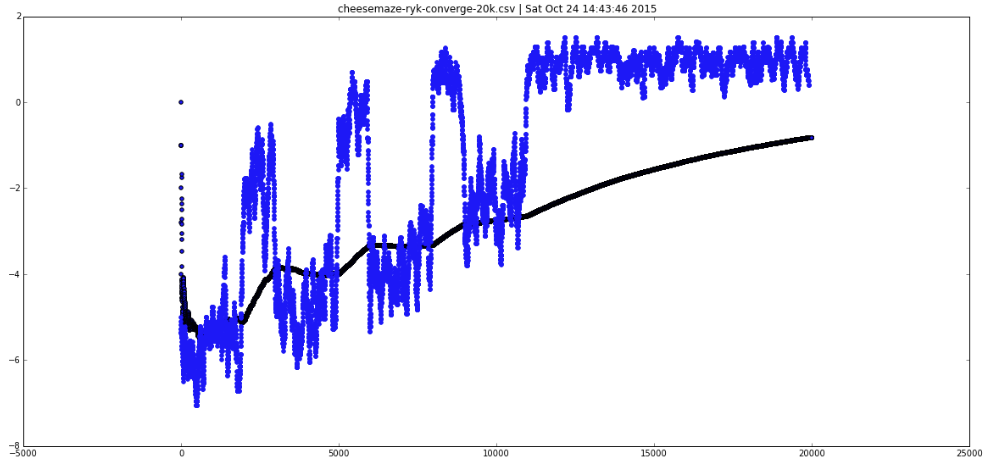
\includegraphics[scale=0.4]{cheesemaze_best} 
\end{figure}


\subsection{Extended Tiger}

Experimental setup ... \\
 Plots ... 


\subsection{Biased Rock-Paper-Scissor}

Experimental setup ... \\
 Plots ... 


\subsection{Tic-Tac-Toe}

Experimental setup ... \\
 Plots ... 


\subsection{Pacman}

Experimental setup ... \\
 Plots ... 


\section{Cross Domain Simulation Results}
\begin{itemize}
\item Cheesemaze and Extended Tiger
\item Cross domain simulation on more difficult environments... 
\item Separate CTW for Obs and Rews...
\end{itemize}

\section{Discussion and Conclusions}


\section*{Appendix}

\appendix

\section{Files}

The report archive should contain the following: 
\begin{verbatim}

MC-AIXI-CTW-Grp3.zip
    \report
        report.pdf // this report
        report.tex
        cheesemaze_01.png // results plots
        extended_tiger_01.png
        biased_rock_paper_scissor_01.png
        tic_tac_toe_01.png
        pacman_01.png
    \src
        main.hpp
        main.cpp
        environment.hpp
        environment.cpp
        agent.hpp
        agent.cpp
        search.hpp
        search.cpp
        predict.hpp
        predict.cpp
        util.hpp
        util.cpp
        README.md
        cheesemaze.conf // environment configuration files
        rockpaper.conf
        tictactoe.conf
        coinflip.conf
        tiger.conf
\end{verbatim}

\section{Grpahs..}

\bibliographystyle{unsrt}
\bibliography{report}

\end{document}
